\documentclass{paper}
\usepackage{hyperref}
\usepackage{datetime}
\usepackage{listings}
\usepackage{graphicx}
\usepackage{float}
\usepackage{hyphenat}
\title{Automated Continious Integration with Travis}
\newdate{date}{24}{02}{2020}
\date{\displaydate{date}}
\author{John Ghatas}

\hypersetup{
    colorlinks=true,
    linkcolor=black,
    urlcolor=red,
    linktoc=all
}

\begin{document}
    % Page 1
    \maketitle
    \newpage
    
    % Page 2
    \tableofcontents
    \newpage

    % Page 3
    \section{Project definition}
    \paragraph{Goal}{This project was pulled from a Lynda tutorial teaching the basics of Docker, 
    the Docker container created runs an express backend using MongoDB as the database server.}

    \section{Running the application}{The first order of business was to ensure that the application
    was able to run locally before deploying it in a Docker container. To do this we ran the following commands in
    the main directory:
    \begin{lstlisting}[language=bash]
        $ npm install
        $ npm start
    \end{lstlisting}
    To start the backend locally \textbf{MongoDB} is required to have a local install. An example of the backen is shown
    in \textbf{Figure \ref{fig:backend}}
    \begin{figure}[!h]
        \centering
        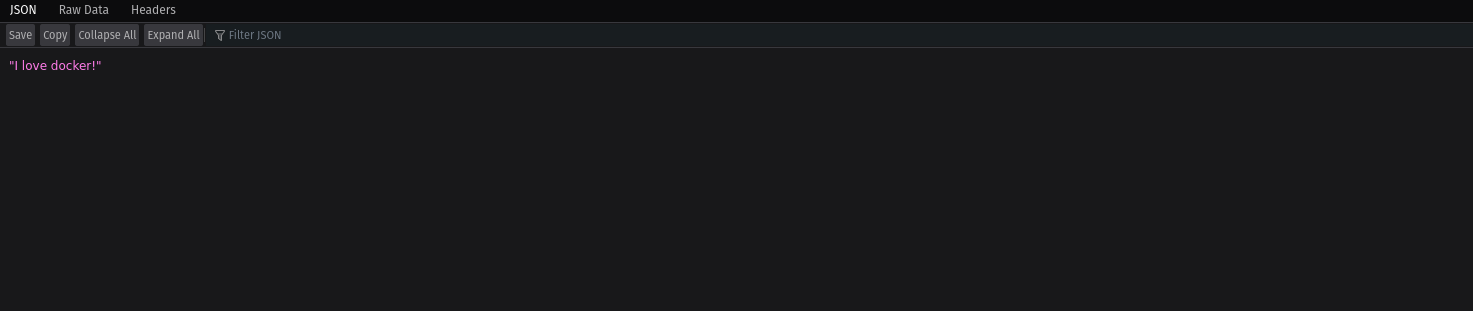
\includegraphics[scale=2.6, pagebox=artbox]{Images/server.png}
        \caption{The root route of the backend running}
        \label{fig:backend}
    \end{figure}
    \newpage
    }

    % Page 4
    \section{Exporting to docker}{
    The next step was to export the image to docker locally, to ensure the setup was
    running before deploying the automation of the Docker image to the TravisCI servers. To build a Docker image, I had to create
    a Dockerfile specifying the steps that needed to be taken to deploy the Express backend in a Docker container. The Dockerfile
    is shown in \textbf{Figure \ref{fig:dockerfile}}.
    \begin{figure}[!h]
        \centering
        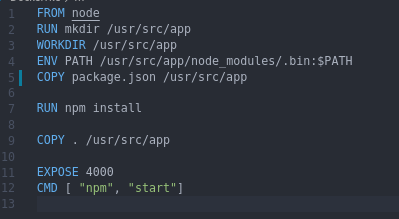
\includegraphics[scale=3, pagebox=artbox]{Images/Dockerfile.png}
        \caption{The dockerfile containing the instructions for building the container}
        \label{fig:dockerfile}
    \end{figure}
    \newline
    To prevent any unnecessary files being transferred to the Docker container, a \textbf{.dockerignore} file is defined.
    We ignored the Node Modules folder and the debug log from the Node Package Manager, thus reducing the total size of 
    the container. Now we could build the image with following command (assuming you are in the root folder of the repository):
    \begin{lstlisting}[language=bash]
        $ docker build . -t [domain]/[name]
        $ docker run -p [local port]:[docker port] 
        -d [domain]/[name]
    \end{lstlisting}
    }    
    \newpage

    % Page 5
    \section{Configuring TravisCI}{Now that I ensured the backend runs locally, we were ready to automate the building 
    of the docker image on Travis. To configure Travis, a \textbf{.travis.yml} file was created to specify the instructions 
    for the CI tool. In \textbf{Figure \ref{fig:travis}} the configuration is shown of the travis file.
    \begin{figure}[!h]
        \centering
        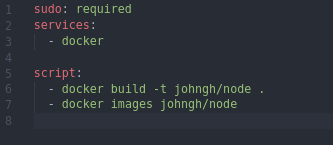
\includegraphics[scale=3, pagebox=artbox]{Images/travis.png}
        \caption{The configuration file of for the CI tool}
        \label{fig:travis}
    \end{figure}
    \newline
    The configuration file will be picked by the plugin TravisCI, that I installed on the repository automating the build. After
    the build is done the status will be updated in the README of the repository as can be seen in \textbf{Figure \ref{fig:result}}.
    \begin{figure}[!h]
        \centering
        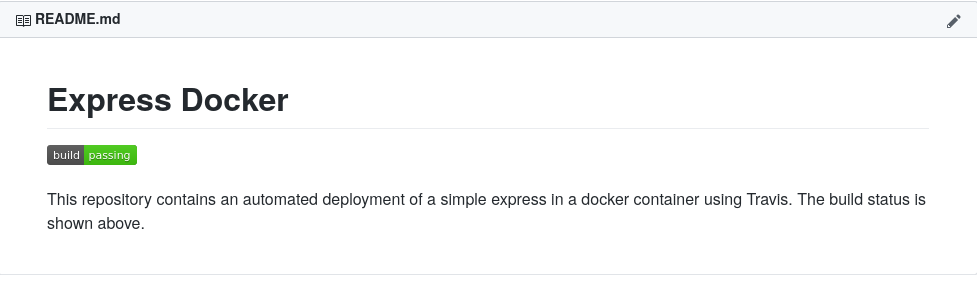
\includegraphics[scale=1.4, pagebox=artbox]{Images/README.png}
        \caption{The build status of the build of the Docker container}
        \label{fig:result}
    \end{figure}
    }

\end{document}